\documentclass[a4paper,12pt]{article}

% Import the deliverable package from common directory
\usepackage{../common/deliverable}

% Tell LaTeX where to find graphics files
\graphicspath{{../common/logos/}{./figures/}{../}}

\usepackage{amsmath}
\usepackage{amssymb}
\usepackage{xspace}
\usepackage{lipsum}
\usepackage{pgfplots}
\usepackage{pgfplotstable}


% Set the deliverable number (without the D prefix, it's added automatically)
\setdeliverableNumber{1.3}

% Begin document
\begin{document}

% Create the title page with the title as argument
\maketitlepage{Report on deal.II improvements}

\newpage

% Main Table using the new environment and command
\begin{deliverableTable}
    \tableEntry{Deliverable title}{Report on deal.II improvements}
    \tableEntry{Deliverable number}{D1.3}
    \tableEntry{Deliverable version}{v1}
    \tableEntry{Date of delivery}{August 31, 2025}
    \tableEntry{Actual date of delivery}{August 28, 2025}
    \tableEntry{Nature of deliverable}{Report}
    \tableEntry{Dissemination level}{Public}
    \tableEntry{Work Package}{WP1}
    \tableEntry{Partner responsible}{SISSA}
\end{deliverableTable}

% Abstract and Keywords Section
\begin{deliverableTable}
    \tableEntry{Abstract}{This report details the progress made during the second semester (Months 7--12) of the dealii-X project in enhancing the deal.II finite element library. The focus is on enhancements for exascale readiness, specifically in high-performance matrix assembly, matrix-free GPU integration, as well as polygonal discretization (to be integrated in the library). Furthermore, this report outlines other relevant enhancements to deal.II undertaken within the project's work packages during this period.}
    \tableEntry{Keywords}{deal.II library; finite element method; Krylov subspace methods; sparse direct solver; matrix-free algorithms; mesh generation; polygonal discretization; CUDA; Kokkos}
\end{deliverableTable}

\newpage

\begin{documentControl}
    \addVersion{0.1}{August 10, 2025}{Andrea Cangiani}{Initial draft}
    \addVersion{0.2}{August 26, 2025}{Andrea Cangiani}{Gathered information from all partners}
    \addVersion{1.0}{August 29, 2025}{Andrea Cangiani}{Final adjustments between partners}
\end{documentControl}

\subsection*{{Approval Details}}
Approved by: M. Kronbichler \\
Approval Date: August 29, 2025

\subsection*{{Distribution List}}
\begin{itemize}
    \item [] - Project Coordinators (PCs)
    \item [] - Work Package Leaders (WPLs)
    \item [] - Steering Committee (SC)
    \item [] - European Commission (EC)
\end{itemize}

\vspace*{2cm}

\disclaimer

\newpage

\tableofcontents % Automatically generated and hyperlinked Table of Contents

\newpage

\section{Introduction}
    \subsection{Overview of the dealii-X Project and Objectives}

The dealii-X project is a pioneering initiative dedicated to developing a
high-performance and scalable computational platform based on the deal.II finite
element library. The project directly addresses the
HORIZON-EUROHPC-JU-2023-COE-03-01 topic, specifically focusing on the
``Personalised Medicine / Digital twin of the human body'' as an Exascale
Lighthouse application area. The overarching goal of dealii-X is to advance
existing pre-exascale digital twin applications for human organs, such as some
deal.II based applications dedicated to the simulation of the brain, heart,
lungs, liver, and cellular interactions, to achieve exascale readiness. 

The project aims to enable real-time simulations of intricate biological
processes, thereby contributing to personalized medicine and cutting-edge
healthcare research. Ultimately, this enhanced simulation capability holds the
potential to significantly improve medical diagnostics and treatment planning.

\subsection{Objectives of Work Package 1 (WP1)}

The main objective of Work Package 1 (WP1) is to serve as the foundation
for the dealii-X Centre of Excellence by enhancing and expanding the
capabilities of the deal.II library to address the challenges of exascale
computing and facilitate the creation of advanced digital twins of human
organs.

The key steps of WP1 include:
\begin{itemize}
    \item Extending and improving the exascale capabilities of deal.II;
    \item Improving pre-exascale modules of the deal.II library;
    \item Developing an experimental polygonal discretization module for deal.II;
    \item Integrating PSCToolkit within deal.II;
    \item Integrating MUMPS within deal.II.
\end{itemize}

Specifically, the sub-work packages aim to:
\begin{itemize}
    \item \textbf{WP1.1 (Lead RUB)}: Develop matrix-free computational methods optimized for GPU architectures and enhance the scalability of solvers;
    \item \textbf{WP1.2 (Lead UNIPI)}: Improve the gmsh API, develop a generalized interface for coupling operators, enhance reduced order modeling capabilities, integrate low-rank approximation methods, and develop block preconditioners;
    \item \textbf{WP1.3 (Lead SISSA)}: Introduce and parallelize polygonal discretization methods within deal.II and develop related multigrid techniques;
    \item \textbf{WP1.4 (Lead UNITOV)}: integrate PSCToolkit into deal.II, leveraging GPU computing and developing efficient preconditioners for multiphysics problems;
    \item \textbf{WP1.5 (Lead INPT)}: Integrate the MUMPS solver directly into deal.II for use in multigrid methods and explore low-rank and mixed-precision techniques;
\end{itemize}

In summary, WP1 is dedicated to developing and integrating fundamental software components within the deal.II library and external libraries, with a strong emphasis on enabling exascale computation for the digital twin applications in WP2.

\subsection{Purpose and Scope of this Report (Deliverable D1.3)}

The purpose of this second report on Work Package 1 is to present an updated and detailed account of the progress achieved during the six months following the initial reporting period of the dealii-X project. Building upon the foundational activities and strategies outlined in the first report (D1.2), this document focuses on the continued development and refinement of the deal.II library to address the requirements of exascale computing and to further enable the creation of advanced digital twins of human organs.

The scope of this report includes the assessment of technical developments within WP1, with particular emphasis on the optimization and scaling of computational methods, the deepening integration of key external libraries, and the maturation of novel discretization techniques explored during the early stages. It also covers the collaborative efforts across the sub-work packages, highlighting how initial prototypes and concepts have progressed towards more robust and deployable solutions.

The report will document significant milestones reached, pointing to specific related deliverables such as D1.5, challenges encountered in this intermediate phase, and the strategies adopted to overcome them. It will provide a mid-term perspective on the trajectory of WP1 towards its objectives, demonstrating its growing contribution to the overarching goals of the dealii-X project.

As with the first report, quantitative evaluation of WP1's advancement is based on an updated list of pull requests (PRs) and issues recorded in the deal.II GitHub repository, alongside a summary of improvements in related satellite repositories.%, enabling a clear measurement of technical and collaborative progress since the first reporting period.

\section{Improvements for Exascale Readiness}

Work package 1.1 focuses on enabling efficient finite element computations
with the deal.II finite element library, where matrix-free evaluation
techniques and multigrid methods are the core scientific components.

\subsection{Objectives and Planned Activities (Task WP1.1.1)}

The primary objective of WP1.1, led by RUB, is to extend the capabilities of deal.II’s matrix-free implementations for modern graphics cards. To test and evaluate the performance of these accelerators, CEED benchmarks \cite{Kolev2021} were implemented. 

\subsection{Progress and Current Status}

The current status of the implementation focuses on element-wise communication-free algorithms such as mass and stiffness matrix operators. 

Implementations are available in the \url{https://github.com/dealii-X/benchmarks} repository. A brief overview of the kernels is provided below:
\begin{itemize}
\item Bake-off Kernel 1 (BK1) for mass-matrix operator on Gauss-Lobatto quadrature points.
\item Bake-off Kernel 5 (BK5) for stiffness-matrix operator on Gauss-Lobatto-Legendre quadrature points.
\end{itemize}

The main challenge in implementing benchmarks on cutting-edge accelerators is the growing number of GPU vendors such as Nvidia, AMD, and Intel, whose non-standard programming models bring an additional burden on developers. To address this, this subproject also aims to ensure portability across different GPUs by employing the Kokkos library~\cite{Trott2022}, which supports multiple back-ends. Accordingly, current implementations evaluate the portability and performance of Kokkos by comparing it with CUDA kernels.


\subsection{Implementation Details}

All implemented GPU kernels follow a common sequence for matrix-free evaluations, which can be described as:
\begin{itemize}
\item[1] Each block/warp is assigned to an element to perform operator evaluation.
\item [2] Each block/warp caches the required interpolation matrices from global memory into shared memory.
\item[3] Each block/warp performs the tensor contractions and stores intermediate values in shared memory.
\item[4] Inserted block/warp-level synchronizations ensure thread safety after each contraction.
\item[5] Element-wise solution vectors are copied back from shared memory to global memory.
\end{itemize}

Certain optimization strategies and algorithmic design choices are partially motivated by the findings of the research~\cite{Swiry2019} in our implementations. Our optimization techniques can be classified based on the four categories;
\begin{itemize}
\item[1] Thread Granularity (block-centric and warp-centric)
\item [2] Thread-level Data Mapping (strided fashion, simple map)
\item[3] Thread Dimension in each Thread-Block (2D and 3D)
\item[4] Compile time and runtime evaluation of number of quadrature points.
\end{itemize}

\subsection{Preliminary Results}

{\bf BK1.} Early performance results for the different test cases are shown in Figures~\ref{fig:BK1_1} and~\ref{fig:BK1_2}, evaluated on an Nvidia H100 GPU. Each test case uses 3D thread blocks, determines the number of quadrature points at run time, and employs thread blocks for element-wise computations. The only difference between the two cases is the programming model: Figure 1 presents the results obtained with CUDA, while Figure 2 shows those from the Kokkos library.
The first finding is that polynomial order 1 shows lower performance compared to higher-order elements in both test cases. This behavior, rooted in a first-order polynomial, is configured with 27 threads per block. This leads to under-utilization of the warp (size 32) on the target hardware.
The second finding is that Kokkos achieves approximately 90\% of the performance observed with the CUDA model, demonstrating that the performance portability model introduces only a minor overhead.

\begin{figure}
\centering
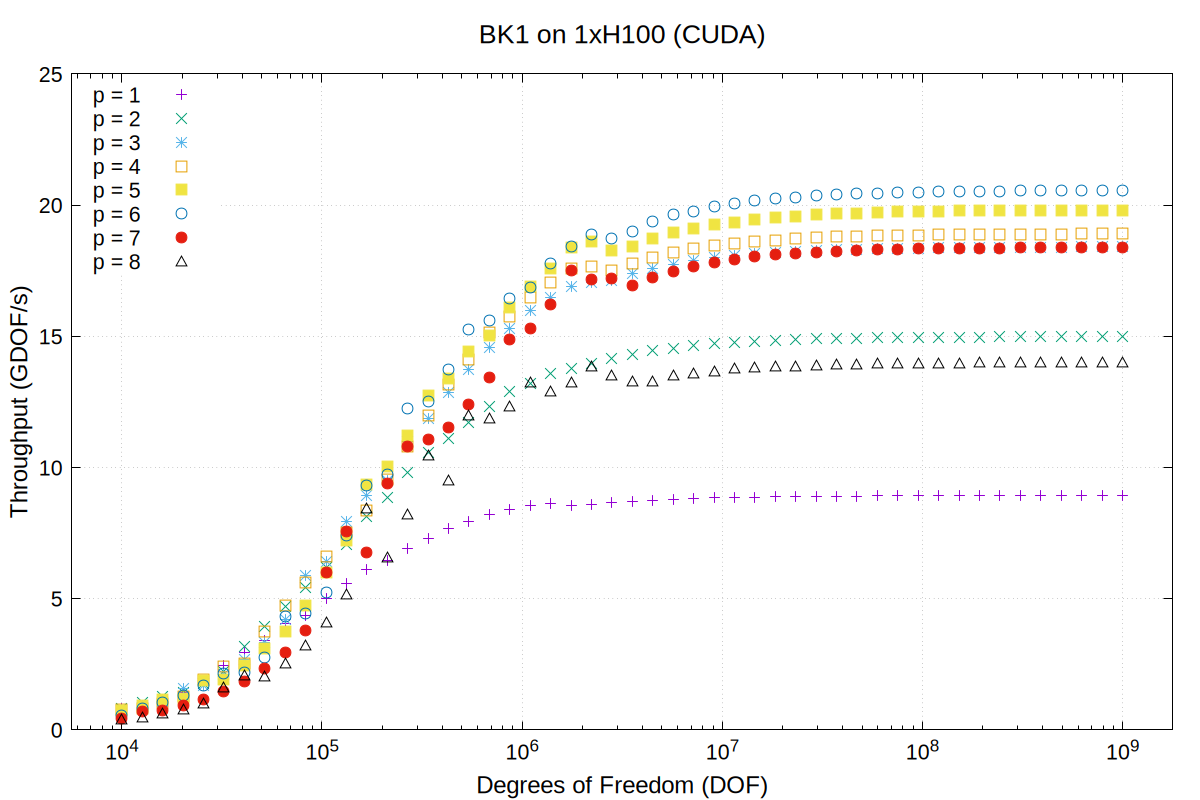
\includegraphics[width=0.8\textwidth]{BK1_1}
\caption{BK1 performance results on Nvidia H100 GPU with CUDA programming model. Various polynomial orders are tested, and saturation of hardware resources is visible after $10^6$ degrees of freedom. Polynomial order 1 performs the worst due to under-occupation of the single warp.\label{fig:BK1_1}
\end{figure}
\begin{figure}
\centering
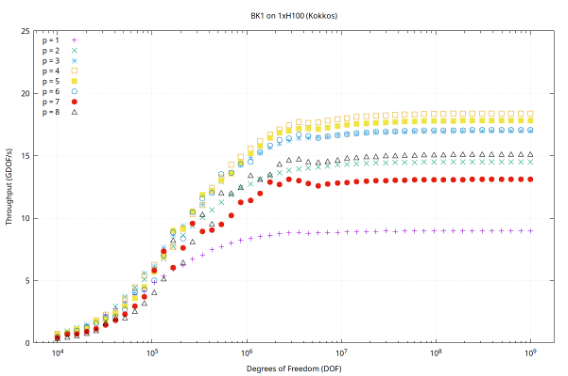
\includegraphics[width=0.8\textwidth]{BK1_2}
\caption{BK1 performance results on an NVIDIA H100 GPU using the Kokkos library. The same test conditions and optimization techniques as in Figure 1 were applied. Kokkos attains nearly 90\% of the performance delivered by CUDA.}
\label{fig:BK1_2}
\end{figure}

{\bf BK5.} Unlike the multiple polynomial order evaluations in the BK1 test cases, we analyzed the kernels with a fixed cubic polynomial order (p=3) and templated quadrature points. Using templates shifts certain computations from runtime to compile-time, allowing the compiler to apply optimizations. As a result, templated implementations are often significantly faster, in most cases improving performance by 30\% at least, compared to their runtime counterparts.

Both CUDA and Kokkos kernels were implemented with three-dimensional thread blocks and a simple data mapping approach, where each thread operates on a single data entry. The total number of degrees of freedom (DOF) in this test case is 27 million. Kernel performance values were measured by NVIDIA Nsight Compute. In these measurements, both CUDA and Kokkos executions completed in 0.71 ms, showing identical performance. Nsight Compute reported an arithmetic intensity of 1.97 FLOP/byte, which places these kernels in the memory-bound region of the roofline model for the H100 GPU. The achieved performance was 5.7 TFLOPs, compared to the hardware limit of 6.6 TFLOPs at this arithmetic intensity. This corresponds to 86\% of peak bandwidth utilization (2.88 TB/s out of 3.2 TB/s). The kernels also achieved 75\% occupancy, and register usage per thread was identified as the primary limiting factor.

Overall, the results demonstrate that both CUDA and Kokkos BK5 implementations deliver near-optimal performance on the H100, efficiently exploiting available memory bandwidth and achieving performance levels very close to the hardware limits.


\section{Improvement of pre-exascale modules of the deal.II library}

Work package 1.2 focuses on enhancing the existing modules of the deal.II
library to prepare them for the challenges of exascale computing. This includes
several key activities: 
\begin{itemize}
    \item Improving the gmsh API to support large-scale;
    \item Developing a generalized interface for coupling operators, which
    is fundamental for multiphysics and multiscale simulations, including methods
    for conforming and non-conforming grids and non-local coupling techniques;
    \item Enhancing the reduced-order modeling (ROM) capabilities of deal.II,
    implementing algorithms for data analysis and reduced-order geometric modeling;
    \item Integrating low-rank approximation methods within deal.II, including
    low-rank and hierarchical low-rank solvers and preconditioners to tackle
    large-scale computational problems;
    \item Developing block preconditioners for coupled problems, which are
    essential for the stability and efficiency of simulations.
\end{itemize}
 
The overall objective is to improve the pre-exascale functionalities of deal.II,
making it an even more robust and efficient library for a wide range of
scientific and engineering applications aiming for the use of exascale
computers.


\subsection{Progress and Current Status}



\section{Polygonal Discretization Methods}

 The dealii-X project Work Package 1.3, lead by the SISSA team, will deliver an experimental module enhancing the
deal.II library with the capability to perform efficiently polygonal discretization, that is numerical methods based on general polygonal and polyhedral meshes.% in place of standard simplicial and hexahedral meshes. 

\subsection{Objectives and Planned Activities (Task WP1.3.1 and WP1.3.2)}

%The primary objective of WP1.3 is the development of a polygonal discretization module within the deal.II library. 
The deal.II library currently
supports a wide range of finite element methods, defined on standard simplicial
and hexahedral meshes, but does not support polygonal and polyhedral (\emph{polytopic}) meshes.
The primary objective of WP1 is the development of a polygonal
discretization module within the deal.II library. The module is designed to be integrated into the deal.II library, and its integration is expected to be completed by the end of the project.

This task requires the development of the basic data structure for polytopic meshes obtained by agglomeration of standard deal.II meshes and the exploitation of such data structure for the implementation of polygonal discretizations.


 \subsection{Progress and Current Status}

The preliminary version of the polygonal discretization module developed within the first six months of the project was made available at https://github.com/fdrmrc/Polydeal.
The module has since been extensively tested and parallelised. 
Milestone M5 has been reached and deployed as deliverable D1.5 (cf. the specific report for more details). The milestone was set to establish the parallel implementation of polygonal discretization methods. The deliverable provides a tutorial program on polygonal discretizations, showcasing the implementation of these methods for the solution of a basic model problem. Aside from the tutorial, a series of problems and tests have been run, confirming the validity and robustness of the approach for the solution of problems in the dimension-independent setting. In particular, the polytopic discontinuous Galerkin methods have been implemented for the solution of a series of benchmark problems, including fluid mechanics and electrophysiology.


{\bf Fluid mechanics.}
The polytopic discontinuous Galerkin method has been extended to the solution of fluid mechanics boundary value problems with the analysis of the method for the solution of the Oseen problem. This required a new analysis which has been carried out for the $hp$-version of the method, hence permitting arbitrarily high-order implementations. Both stabilised equal order $(\mathcal{P}_k,\mathcal{P}_{k})$ and pressure lower-order $(\mathcal{P}_k,\mathcal{P}_{k-1})$ versions have been analysed. 
New working examples implementing the new method have been committed by the SISSA team within the examples suits of the {\em polydeal} repository \url{https://github.com/fdrmrc/Polydeal}.
% https://github.com/fdrmrc/Polydeal/blob/main/examples/darcy_stokes.cc
Preliminary results show that the polytopic discontinuous Galerkin (polyDG) is achieving the optimal convergence rate when applied to the Oseen problem. Using the \emph{polydeal} data structure, a sequence of polygonal meshes obtained by agglomeration of a single fine quadrilateral mesh has been created, see Figure~\ref{fig:metis}. The corresponding results shown in Table~\ref{tab:meshes} display the corresponding convergence rate achieved by the polyDG method solving a model problem for the Oseen equation with variable coefficients.
\begin{figure}[!htb]
\centering
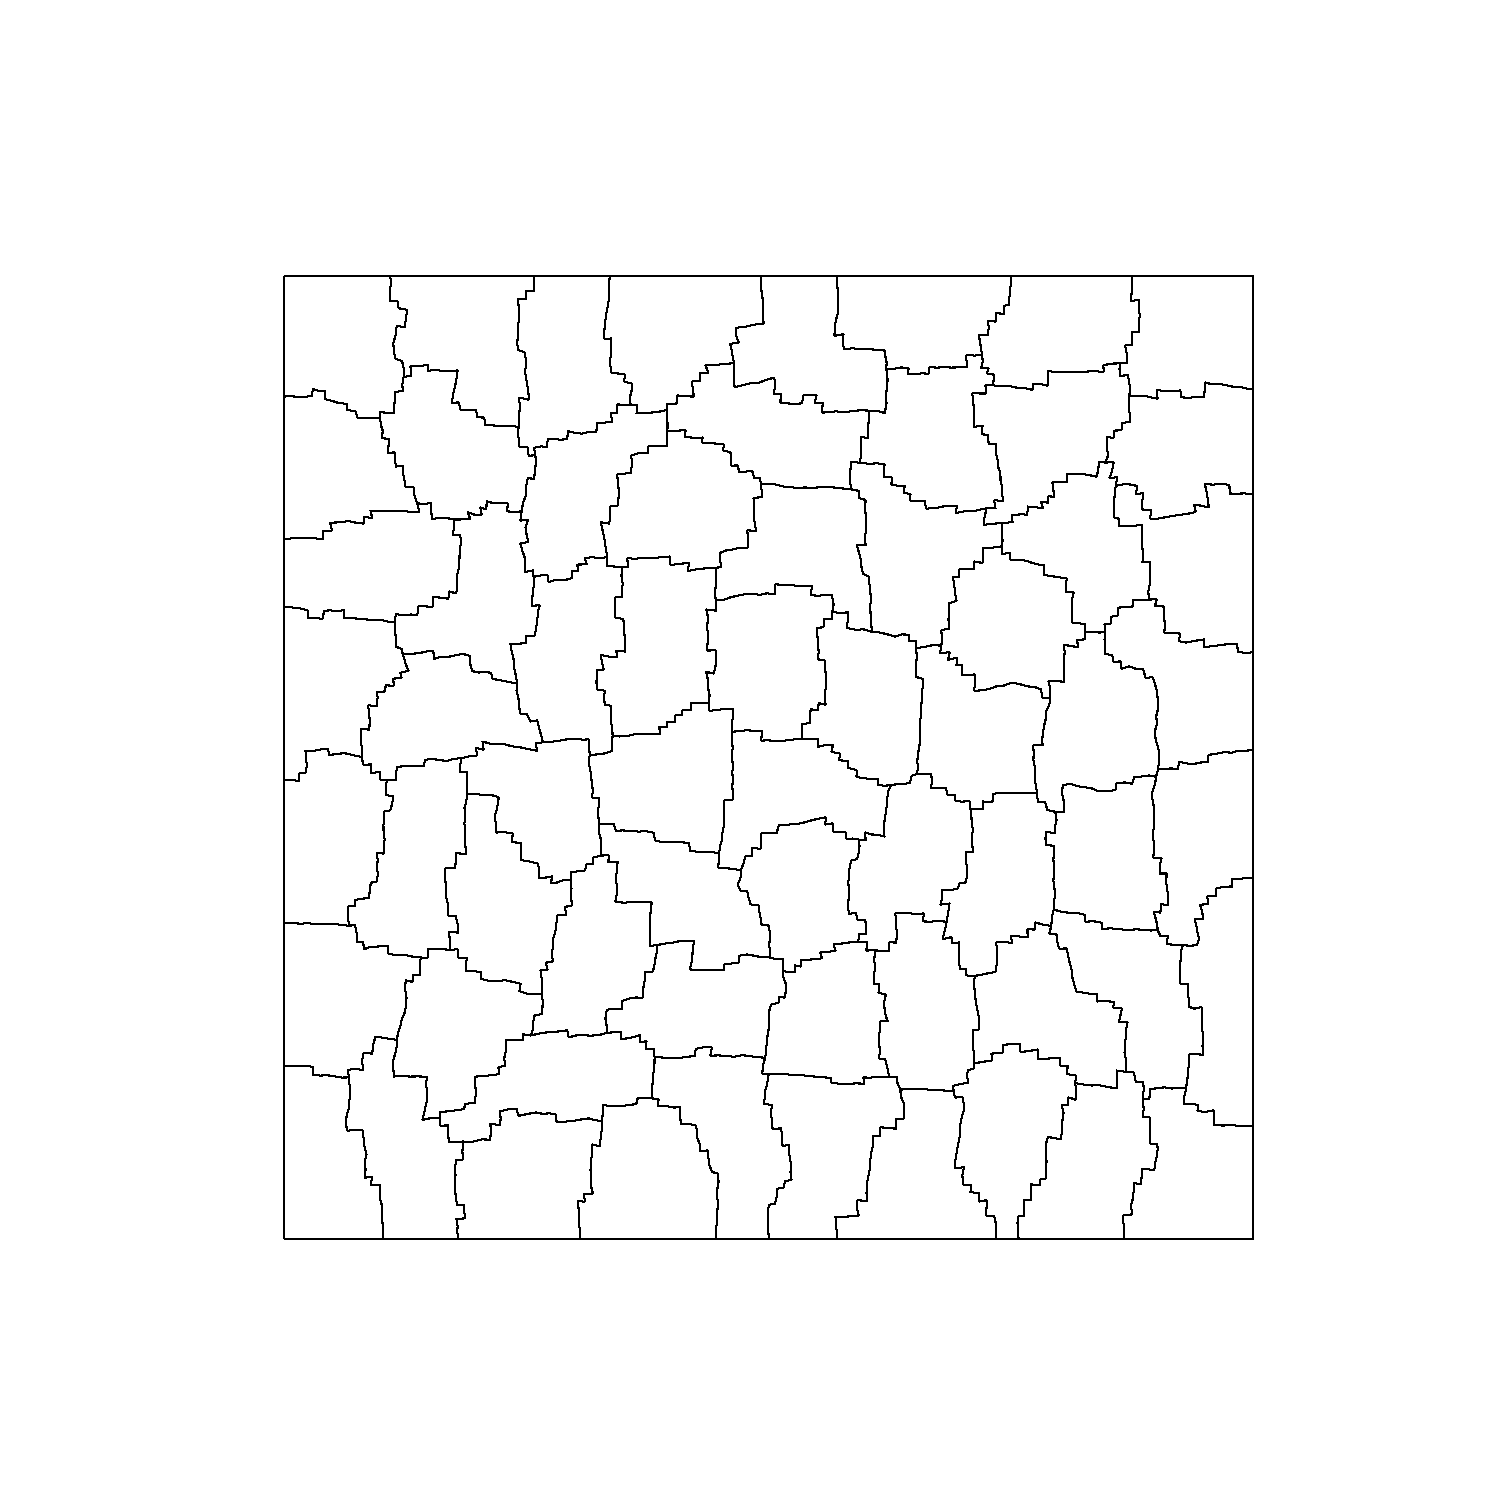
\includegraphics[height=0.3\linewidth]{metis_level3}
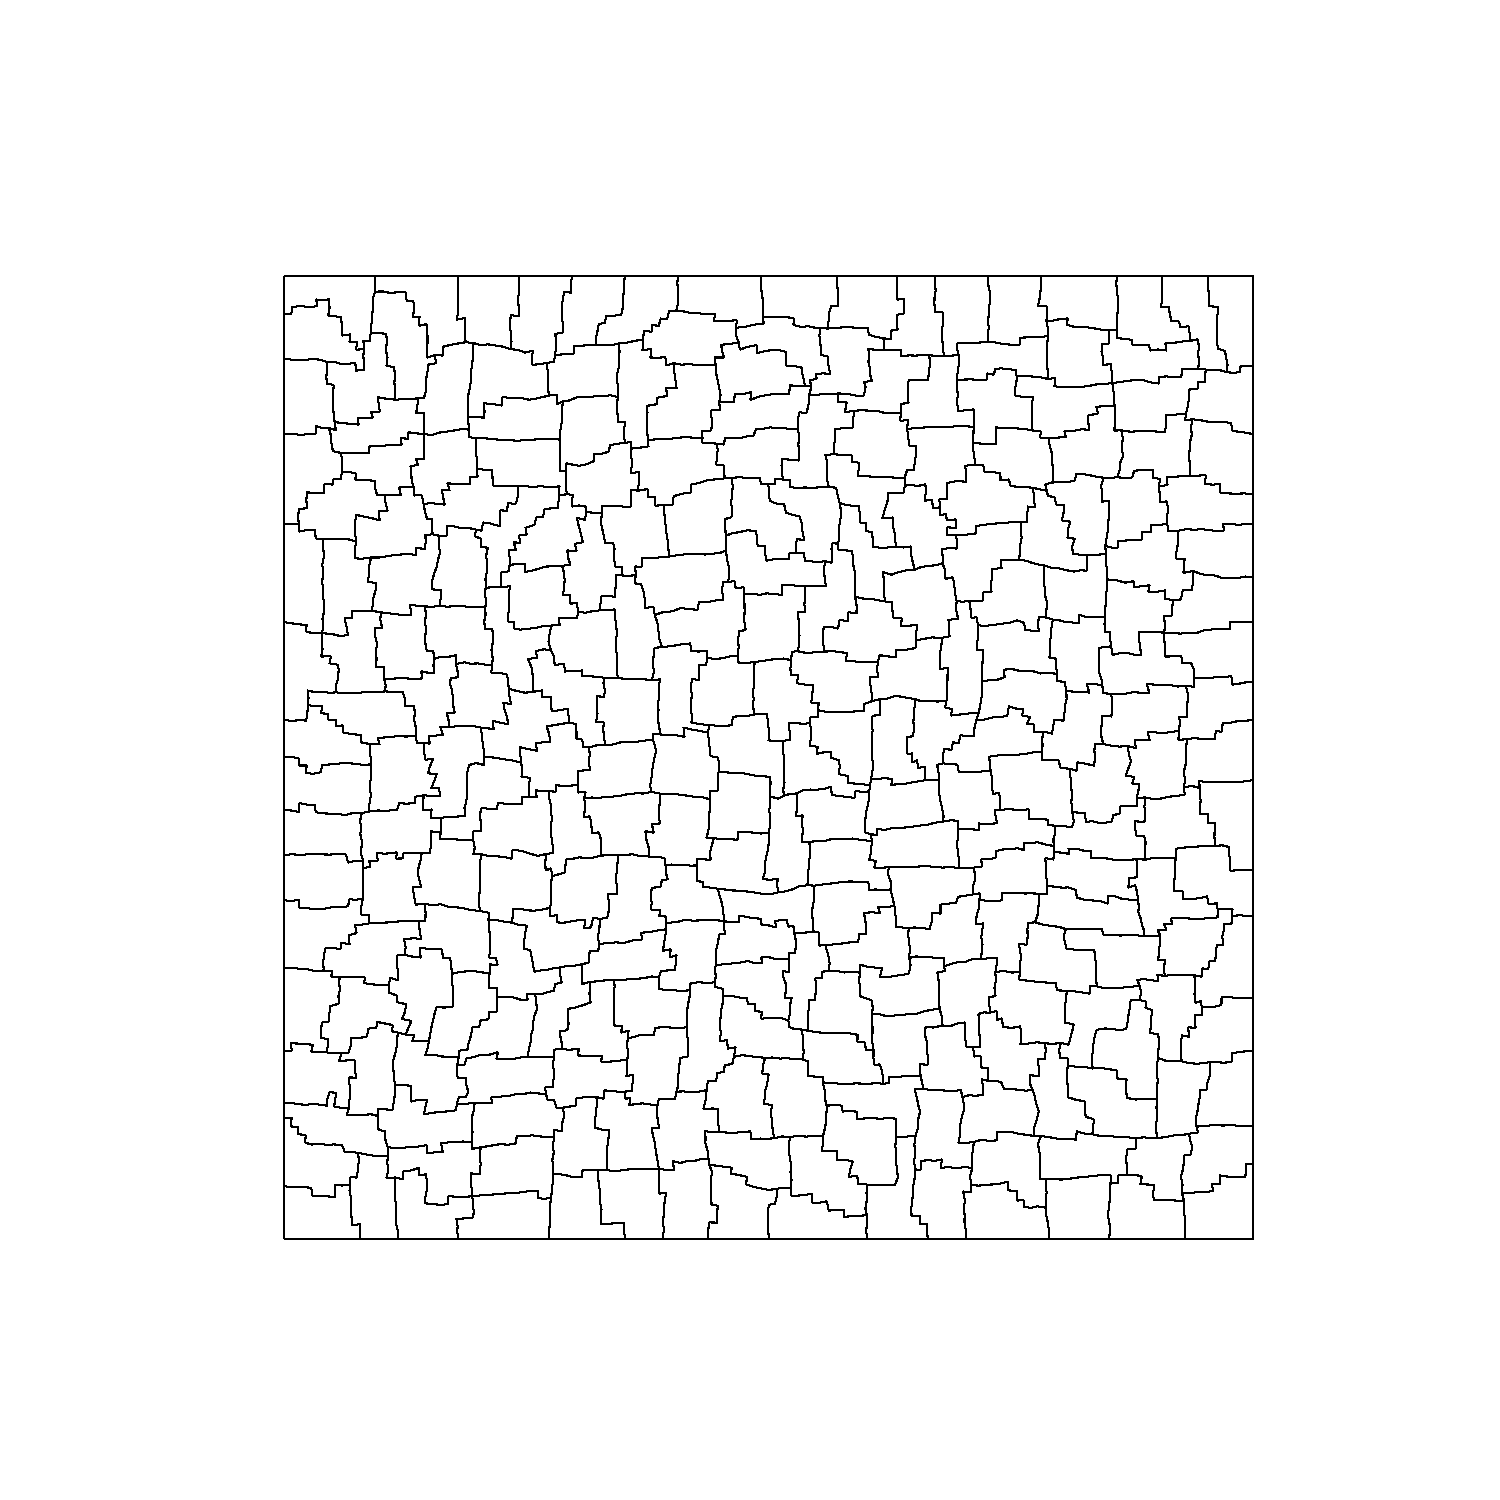
\includegraphics[height=0.3\linewidth]{metis_level4}
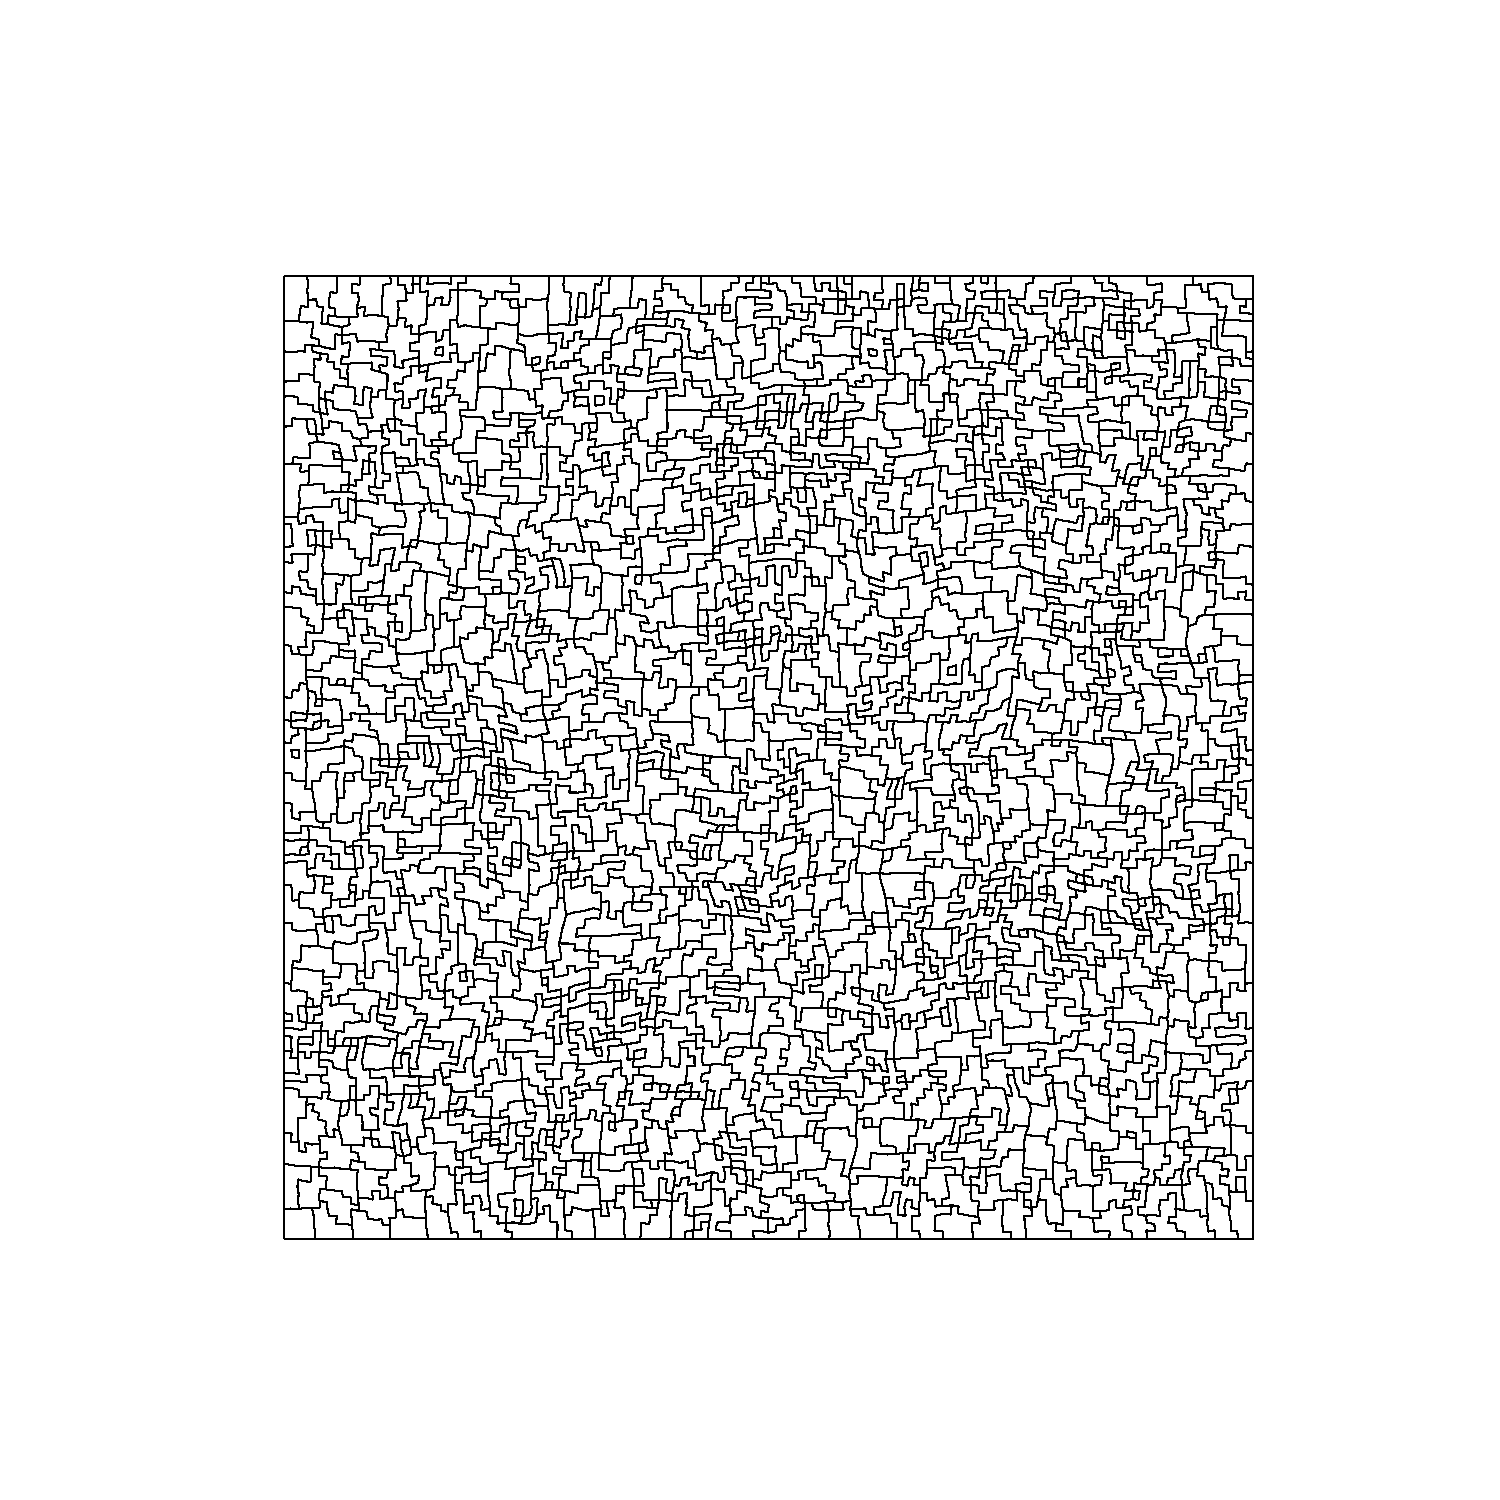
\includegraphics[height=0.3\linewidth]{metis_level5}
\label{fig:meshes}
\caption{Three subsequent levels of the meshes obtained by METIS-based agglomeration of an underlying fine quadrilateral mesh.}
\end{figure}
\begin{table}[!ht]\centering
\caption{Energy-norm errors and convergence orders for an Oseen test problem with variable coefficients and $Re=1$ in function of the agglomeration level for the meshes sampled in Figure~\ref{fig:meshes}.}
\label{tb1}
{\small
\begin{tabular}[c]{cc|cc}\hline\hline%\cline{3-8}
&{Level}&energy-norm error&order\\ \hline
{$\mathcal{P}_2$-$\mathcal{P}_2$}
&4 &7.69E-00&1.86\\
&5 &2.46E-00&1.64\\
&6 &6.50E-01&1.92\\
&7 &1.17E-01&2.48\\
\hline
{$\mathcal{P}_3$-$\mathcal{P}_2$}
&4 &1.16E-00&2.70\\
&5 &2.14E-01&2.44\\
&6 &3.21E-02&2.73\\
&7 &2.68E-03&3.58\\
\hline\hline
\end{tabular}}
\label{tab:oseen}
\end{table}
A publication presenting both the new sharp a priori analysis of the discontinuous Galerkin method for the Oseen problem as well as numerical experiments validating the approach for the solution of the Oseen problem is under preparation. It will be submitted to a top numerical analysis journal within the next semester.


 \subsection{Challenges and Future Plans}

Before integration into the deal.II library, additional testing and generalization are necessary to demonstrate the potential of polygonal discretization in solving the same range of models currently supported by standard finite elements. Moreover, further work on efficient implementation is required to fully exploit the complexity-reduction capabilities of these methods. This effort will include, for example, the automatic construction of coarse polygonal grid hierarchies and mesh adaptivity algorithms, as well as the development of advanced solvers, such as multigrid techniques, which constitute the next phase of the project.


\section{Integration of PSCToolkit into deal.II (WP1.4)}
    \subsection{Objectives and Planned Activities}
        The primary objective of WP1.4 is to integrate the PSCToolkit (Parallel Sparse Computing Toolkit) into the deal.II library. This integration aims to leverage GPU computing to enhance performance and develop efficient preconditioners for multiphysics problems. PSCToolkit provides advanced routines for sparse matrix operations optimized for GPU architectures, which are critical for large-scale simulations.

        Planned activities include:
        \begin{itemize}
            \item Developing a GPU-accelerated interface for PSCToolkit within deal.II;
            \item Implementing efficient preconditioners tailored for multiphysics problems;
            \item Benchmarking the performance of the integrated toolkit on exascale systems.
        \end{itemize}

        \subsection{Progress and Current Status}
 
The activities at UNITOV have centered around the integration of PSCToolkit solvers into the deal.II framework; our work has been conducted with close coordination with UNIPI. 
To interface PSCToolkit we have had to 
Redefine some interfacing machinery on PSCToolkit side:
\begin{itemize}
\item Complete CMAKE build support:
\item Upgrading the SUNDIALS interface.
\end{itemize}
The use of PSCToolkit into deal.II is planned through the availability of a SUNDIALS/KINSOL interface: deal.II makes calls into KINSOL/SUNDIALS, which in turn calls into PSCToolkit. Previous releases of PSCToolkit had already been interfaced with SUNDIALS, but we had to tackle the upgrades needed for using a new version towards which the entire infrastructure is transitioning. 

Many “small” issues had to be tackled, including: 
Converting the error codes;
Changing the interlanguage (c/c++/Fortran) of complex data;
Making certain configuration parameters available to deal.II code;
Ensuring a complete CMake build could be achieved cleanly;
Defining some additional computational kernels;
Some preliminary testing of the PSCToolkit interface has already taken place.
We are now in a position to start building and testing in the context of the entire application.
The updates have been included in the release candidates for the PSCToolkit component PSBLAS 3.9.0-rc3 and AMG4PSBLAS 1.2.0-rc3.



\section{Integration of MUMPS Solver into deal.II (WP1.5)}
    \subsection{Objectives and Planned Activities}
    WP1.5 aims to integrate the MUMPS (Multifrontal Massively Parallel Sparse) solver directly into deal.II. This task focuses on enabling its use in multigrid methods and exploring advanced techniques such as low-rank approximations and mixed-precision computations to enhance solver efficiency.

    Planned activities include:
    \begin{itemize}
        \item Developing a direct interface between deal.II and MUMPS;
        \item Implementing low-rank approximation techniques to reduce computational costs;
        \item Exploring mixed-precision strategies to optimize performance on modern hardware.
    \end{itemize}

    \subsection{Progress and Current Status}
  In the last semester our activity was focused towards the integration of the MUMPS solver within the deal.II software. The deal.II package used to support a direct MUMPS integration in the past. This support was subsequently removed in favor of an indirect use of MUMPS through the PETSc library. As a first step towards the objectives of WP1 of the dealii-X
project, this support was reverted and improved. The MUMPS interface in deal.ii was extended to support distributed memory parallelism through the use of distributed matrix and vector datatypes as defined in the deal.ii PETSc and Trilinos wrappers. This allows for a completely parallel initialization of the MUMPS data structure (that includes the system matrix and the right-hand sides) prior to the symbolic analysis, numerical factorization and forward/backward substitution. This ultimately allows for the solution of problems of a much larger size. Setting-up MUMPS internal configuration parameters was not possible in original
deal.II MUMPS interface which, therefore, had to be extended to enable the use of the more advanced features of the MUMPS solver; these include the Block Low-Rank approximations, the GPU support and numerous other parameters that allow for fine-tuning both the performance and the numerical robustness of the solver. The full details of this work and the corresponding software documentation are reported in deliverable D1.1.

\bibliographystyle{abbrv}
%\bibliography{../common/bibliography.bib}
\bibliography{bibliography.bib}
    
%\label{MyLastPage}


\end{document}
